% ============================================================================
% Evaluation Protocol Flaws in Facial Kinship Verification
%
% All numeric claims in this manuscript trace to results/honest/*.json and are
% reproducible via scripts/evaluation/run_kfold.py. Do not add a figure or a
% baseline row without a verifiable source.
% ============================================================================

\documentclass[journal,12pt]{IEEEtran}

\usepackage{amsmath,amssymb,amsfonts}
\usepackage{graphicx}
\graphicspath{{figures/}}
\usepackage{booktabs}
\usepackage{multirow}
\usepackage{url}
\usepackage[hidelinks]{hyperref}

\begin{document}

\title{Person-Level Kinship Verification: Leakage-Free Evaluation, Set-Based
Aggregation, and a Negative Result for Quantum-Inspired Metrics}

\author{Sasi~Vaibhav% <-- add co-authors and affiliation before submission
\thanks{Code and data-processing scripts:
\url{https://github.com/svaibhav-7/Quantum_kinship_verification}}}

\maketitle

\begin{abstract}
Facial kinship verification is evaluated almost exclusively as a
photograph-versus-photograph decision on four benchmarks. We argue that this
formulation is both harder to measure reliably and weaker than the data
supports. First, we quantify the leakage admitted by conventional splitting:
because Families In the Wild draws $57{,}120$ pairs from $95$ families and
$472$ identities, a random pair-level split places an identity from
\emph{every} test pair into the training set, a violation we measure at
$11{,}424/11{,}424$ ($100\%$). We propose a leakage-free protocol based on
grouped $k$-fold cross-validation in which every family is tested exactly once
and negatives are regenerated within each fold; this reduces seed-to-seed
accuracy variation from $22.5$ to $12.1$ points. Second, we show that the
conventional formulation discards most of the available evidence: FIW supplies
a median of five photographs per identity, yet the standard protocol scores one
against one. Representing each \emph{person} by their photograph set, as
template-based face recognition does, improves ROC-AUC by $+0.077$ on FIW under
the leakage-free protocol, while reducing exactly to the single-image case on
corpora storing one photograph per person. We further show that scoring
father--mother--child triads jointly, rather than as independent pairs, adds
$+0.032$ ROC-AUC on TSKinFace ($p = 0.0001$). Finally we report a systematic
negative result: nine quantum-inspired formulations, spanning similarity
measures, feature extractors and inductive biases, each evaluated against a
capacity-matched classical control, fail to improve on their controls, and four
are significantly worse. We further show that both findings replicate under a second backbone
(ArcFace), where the person-level gain is larger still ($+0.098$), and we
document a subgroup artefact of independent methodological interest: an
apparent $0.28$ ROC-AUC deficit for mother--son pairs proves to be a
single-family effect that disappears ($0.031$ spread) once no family is allowed
to dominate a fold. All protocol and evaluation code,
together with the JSON artefacts underlying every figure and table, is
released.
\end{abstract}

\begin{IEEEkeywords}
Facial kinship verification, evaluation protocol, dataset bias, data leakage,
quantum-inspired machine learning, negative results.
\end{IEEEkeywords}

% ---------------------------------------------------------------------------
\section{Introduction}

Facial kinship verification asks whether two facial images depict biologically
related individuals. Progress is measured on a small set of public benchmarks,
and reported accuracies have risen steadily. This paper examines whether the
evaluation protocols supporting those numbers are sound.

We make three contributions, of which the first two concern how the task is
posed and measured rather than which model is applied to it.

\textbf{A leakage-free protocol, and the leakage it removes.} Splitting a
corpus at the level of \emph{pairs} rather than \emph{identities} does not
isolate a test set. FIW draws $57{,}120$ pairs from only $95$ families and
$472$ identities, so identities recur across pairs an average of $242$ times;
under a random pair-level split we measure that $100\%$ of test pairs share an
identity with training. Correcting this is less direct than it appears, because
every negative pair joins two families and, treating families as vertices,
yields a graph with a single connected component over all of FIW: no
family-disjoint partition of the existing pairs exists, and negatives must be
regenerated within each fold. That kinship datasets carry construction
artefacts is known --- prior work has shown that negatives assembled by
recombining family members admit shortcuts~\cite{dawson2018samephoto} --- but we are
not aware of a quantification of identity leakage under the splitting practice
in common use, nor of a released protocol that removes it.

\textbf{Person-level rather than photograph-level verification.} The
conventional formulation compares two photographs. FIW supplies a median of
five photographs per identity, so this discards most of the evidence about each
person. Template-based protocols in face recognition score a person represented
by an image set~\cite{whitelam2017ijbb}. Image sets have been used in kinship
verification to learn a set-to-set metric~\cite{kohli2019imageset}; what we
evaluate is different and simpler --- aggregating a subject's photographs into
a single template scored by an ordinary pairwise decision --- and, to our
knowledge, it has not been measured under a leakage-free protocol. Doing so
improves ROC-AUC by $+0.077$ on FIW, and by construction leaves corpora with
one photograph per person unchanged.
We additionally show that father--mother--child triads carry information that
pairwise decomposition destroys, worth a further $+0.032$ ROC-AUC.

\textbf{A negative result for quantum-inspired metrics.} Quantum-inspired
similarity has been proposed for this task. We evaluate nine formulations
against capacity-matched classical controls; none improves on its control and
four are significantly worse. We give a structural account of why, rather than
attributing the outcome to implementation.

Concretely we contribute: (i) a measured quantification of identity leakage
under conventional splitting, and a released protocol that removes it;
(ii) person-level and triadic formulations of the task, with gains measured
under that protocol; and (iii) a pre-registered nine-formulation negative
result for quantum-inspired metrics.

% ---------------------------------------------------------------------------
\section{Related Work}

\subsection{Kinship verification}

Early work framed the task as metric learning, learning a projection under
which related faces lie closer than unrelated ones~\cite{lu2014neighborhood}.
Subsequent methods replaced the hand-designed metric with deep pairwise
encoders and, more recently, attention- and graph-based
architectures~\cite{zhu2022kinship}. Evaluation is concentrated on four
corpora: KinFaceW-I and KinFaceW-II~\cite{lu2012kinfacew},
TSKinFace~\cite{qin2015tri}, and Families In the Wild~\cite{robinson2018fiw},
the last also underpinning the RFIW challenge series~\cite{robinson2020rfiw}.

Reported accuracies are obtained under each dataset's official protocol. We
therefore do not tabulate them against our results: Section~\ref{sec:bias}
shows that those protocols admit two forms of optimistic bias, so a direct
ranking would mislead in both directions.

\subsection{Evaluation bias in vision benchmarks}

That benchmark protocols can inflate reported performance is established in
adjacent fields. Face recognition distinguishes subject-disjoint from random
splitting precisely because identity overlap leaks
information~\cite{kemelmacher2016megaface}, and template-based protocols such as
IJB-B/C score a \emph{person} represented by several images rather than a
single photograph~\cite{whitelam2017ijbb}. More generally, models exploit
incidental correlations in preference to the intended signal, a failure mode
catalogued as shortcut learning~\cite{geirhos2020shortcut} and, earlier, as
dataset bias~\cite{torralba2011unbiased}.

Both concerns apply directly to kinship verification. Construction artefacts in
kinship corpora have been reported~\cite{dawson2018samephoto}, but we are not aware
of a quantification of identity leakage under the splitting practice in common
use, nor of a person-level protocol for this task: existing multi-image work
addresses image-set subspace representations or matching within family
photographs, which is a different problem from aggregating a subject's
photographs into a single template for pairwise kinship
decisions~\cite{kohli2019imageset}. Sections~\ref{sec:bias}
and~\ref{sec:setlevel} address both gaps.

\subsection{Quantum-inspired machine learning}

Quantum feature maps embed classical data in a Hilbert space where inner
products act as kernels~\cite{schuld2019quantum}, with reported gains on
classical tasks~\cite{havlicek2019supervised}. Related lines use SWAP-test
state fidelity as a similarity measure and density matrices as classifiers.
Such methods have been proposed for kinship verification, and the claim that
they outperform classical counterparts on classical data is contested;
dequantization results show that several purported advantages
vanish under scrutiny~\cite{tang2019quantum}.

Section~\ref{sec:quantum} contributes to that debate empirically, evaluating
nine formulations against capacity-matched classical controls.

% ---------------------------------------------------------------------------
\section{Datasets and Experimental Setup}
\label{sec:data}

We use the four corpora on which facial kinship verification is conventionally
evaluated. Table~\ref{tab:datasets} characterises them by the two properties
that govern this work: how many grouping units are available for a
leakage-free split, and how many photographs each stores per individual.

\begin{table}[t]
\caption{The four benchmark corpora. Photographs per identity is the property
that determines whether person-level aggregation is possible at all.}
\label{tab:datasets}
\centering
\small
\begin{tabular}{lrrrr}
\toprule
Corpus & Pairs & Families & Identities & Photos/id. \\
\midrule
KinFaceW-I & 1{,}066 & 533 & 1{,}066 & 1.00 \\
KinFaceW-II & 2{,}000 & 1{,}000 & 2{,}000 & 1.00 \\
TSKinFace & 2{,}236 & 559 & 1{,}677 & 1.00 \\
FIW & 57{,}120 & 95 & 472 & 5.28 \\
\bottomrule
\end{tabular}
\end{table}

Two features drive the rest of the paper. FIW draws $57{,}120$ pairs from only
$95$ families and $472$ identities --- $121$ pairs per identity --- which is
what makes pair-level splitting leak so completely. And only FIW supplies
multiple photographs per individual, so it is the sole corpus on which
person-level aggregation can differ from the conventional formulation. We
report per corpus rather than averaging, because an average over these four
would conceal exactly that asymmetry.

All experiments use a single frozen backbone: FaceNet (Inception-ResNet-v1)
pretrained on VGGFace2, producing $512$-dimensional $\ell_2$-normalised
embeddings. Holding it fixed isolates the protocol and representation questions
from representation-learning effects, and bounds the claims accordingly
(Section~\ref{sec:limitations}).

Every numeric claim derives from JSON artefacts written by the evaluation
scripts, and each experiment is deterministic given its seed: repeated runs
reproduce the reported figures to four decimal places. The implementation
carries 138 tests, including assertions that no grouping unit spans a fold
boundary.

% ---------------------------------------------------------------------------
\section{Sources of Optimistic Bias}
\label{sec:bias}

\subsection{Identity leakage under pair-level splitting}

Let $\mathcal{P}$ be a set of labelled pairs and $\mathrm{id}(\cdot)$ the
identity depicted in an image. A split $(\mathcal{P}_{\text{tr}},
\mathcal{P}_{\text{te}})$ is \emph{identity-disjoint} if
\begin{equation}
\Big(\bigcup_{p \in \mathcal{P}_{\text{tr}}} \mathrm{id}(p)\Big) \cap
\Big(\bigcup_{p \in \mathcal{P}_{\text{te}}} \mathrm{id}(p)\Big) = \emptyset .
\end{equation}
Random splitting over $\mathcal{P}$ does not enforce this. Table~\ref{tab:leak}
reports the measured violation on FIW.

\begin{table}[t]
\caption{Identity leakage under a random $80/20$ pair-level split of FIW.}
\label{tab:leak}
\centering
\resizebox{\columnwidth}{!}{%
\begin{tabular}{@{}lr@{}}
\toprule
Quantity & Value \\
\midrule
Pairs & 57{,}120 \\
Distinct families & 95 \\
Distinct identities & 472 \\
Mean appearances per identity & 242 \\
Largest family, share of all pairs & 19\% \\
\midrule
Test pairs sharing an identity with train & 11{,}424 / 11{,}424 (100\%) \\
Test pairs whose family was seen in train & 11{,}424 / 11{,}424 (100\%) \\
\bottomrule
\end{tabular}%
}
\end{table}

\begin{figure*}[t]
\centering

\includegraphics[width=\textwidth]{fig_leakage}
\caption{(a) Identity leakage on FIW: under conventional pair-level splitting
every test pair shares an identity with training, which the family-disjoint
protocol reduces to zero. (b) The family-size distribution that makes a single
split unstable --- the largest family alone accounts for $19\%$ of all pairs.}
\label{fig:leakage}
\end{figure*}

\subsection{A non-obvious obstacle to correcting it}

Splitting on families is not sufficient by itself. Each \emph{negative} pair
joins two families, and treating families as vertices and negatives as edges
yields a graph over FIW with a single connected component containing all $95$
families. No family-disjoint partition of the existing pairs exists. Negatives
must therefore be discarded and regenerated \emph{within} each side after the
split. We found this empirically: a splitter that passed synthetic unit tests
failed on the real corpus for exactly this reason.

A second consequence is data loss. Because pre-existing negatives straddle any
group boundary, naively dropping them removes usable data --- on KinFaceW-I,
$173$ of $1{,}066$ pairs, leaving only $119$ test pairs. Regenerating negatives
per side instead recovers the test set to $212$ pairs on KinFaceW-I and $400$ on
KinFaceW-II.

\subsection{Family membership as a predictor in TSKinFace}

That kinship benchmarks carry construction artefacts is established. Prior work
has shown that negatives assembled by recombining members of family photographs
permit a model to succeed without learning
kinship~\cite{dawson2018samephoto}, and the TSKinFace protocol documents its own
negative-construction procedure~\cite{qin2015tri}. We do not claim to be the
first to observe that this dataset family is vulnerable.

The specific regularity we measure is distinct from the same-photograph effect,
and worth separating. TSKinFace stores one cropped face per family member, so
\emph{no} pair --- positive or negative --- shares a source photograph, and the
same-photograph shortcut cannot arise. What does hold is that all $800$
positives are drawn within a family and all $800$ negatives across families, so
family membership predicts the label perfectly. A model can exploit correlated
capture conditions --- illumination, camera, background --- shared by members
photographed together.

To measure the margin this affords, we rebuild the negatives so that half are
drawn \emph{within} a family, pairing father against mother: co-photographed,
hence sharing every session cue, but not kin.

\begin{table}[t]
\caption{TSKinFace pair construction. Under the standard protocol family
membership predicts the label perfectly; no pair shares a source photograph in
either construction.}
\label{tab:ts}
\centering
\resizebox{\columnwidth}{!}{%
\begin{tabular}{@{}lccc@{}}
\toprule
Construction & Same-fam.\ pos. & Same-fam.\ neg. & Cosine AUC \\
\midrule
Standard & 100\% & 0\% & 0.7278 \\
Shortcut-free (ours) & 100\% & 50\% & 0.6880 \\
\bottomrule
\end{tabular}%
}
\end{table}

The $0.0398$ ROC-AUC reduction is measured on raw embeddings without training,
so it reflects separability available to any model rather than a property of
ours. All TSKinFace results in this paper use the shortcut-free construction.

We check separately that our FIW results do not rest on the same-photograph
effect that prior work identifies: $8.2\%$ of FIW positives are drawn from a
single source photograph (against $0\%$ of negatives), and excluding them
changes accuracy by $+0.08$ points ($82.53\% \to 82.61\%$). The effect is
present in FIW but our model does not exploit it.

% ---------------------------------------------------------------------------
\section{Corrected Protocol}
\label{sec:protocol}

We adopt grouped $k$-fold cross-validation with $k=5$. The grouping unit is the
family, which is the unit that shares identities and capture conditions.

\begin{enumerate}
\item \textbf{Positives only are partitioned.} Families are dealt largest-first
into the currently smallest fold, which keeps folds balanced despite the highly
skewed family sizes.
\item \textbf{Negatives are generated per side}, after partitioning, from the
families present on that side.
\item \textbf{Group keys are dataset-scoped.} The family identifier
\texttt{fd\_003} occurs in both KinFaceW-I and KinFaceW-II denoting different
families; an unscoped key merges them and corrupts the disjointness check.
\item \textbf{Family contribution is capped} at $1{,}500$ pairs, preventing the
largest FIW family ($19\%$ of all pairs) from dominating whichever fold it
enters.
\item \textbf{Thresholds are calibrated on a group-disjoint validation slice} of
the training side. The test fold is scored once.
\end{enumerate}

Fold integrity is verified directly rather than assumed: zero folds exhibit
train/test group overlap, and every family is tested exactly once with no
duplicates ($95/95$ FIW, $533/533$ KinFaceW-I, $1000/1000$ KinFaceW-II,
$559/559$ TSKinFace).

\subsection{Effect on measurement stability}

\begin{figure}[t]
\centering
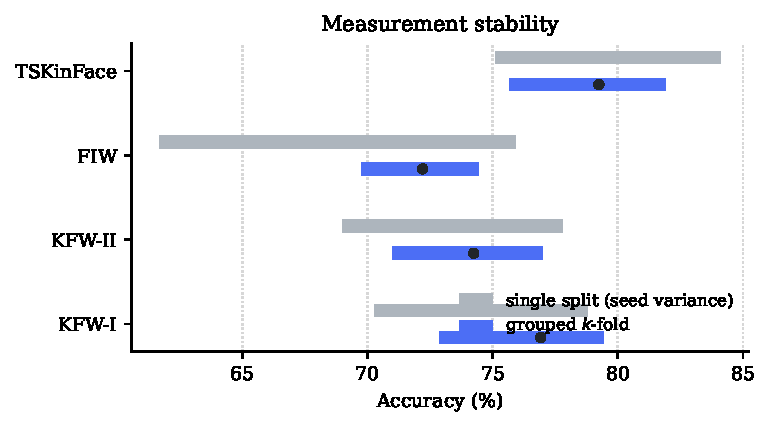
\includegraphics[width=\columnwidth]{fig_stability}
\caption{Accuracy range under a single group-disjoint split across random
seeds (grey) against grouped $k$-fold (blue, mean marked). A single split is
too unstable to support a headline number: on FIW the seed-to-seed range spans
$14.2$ points.}
\label{fig:stability}
\end{figure}

Table~\ref{tab:stab} shows why a single group-disjoint split is insufficient.
Accuracy on one split varies by up to $14.2$ points with the random seed,
because FIW's test side reduces to a small number of families of very unequal
size.

\begin{table}[t]
\caption{Accuracy range across seeds (single split) versus across folds
(grouped $k$-fold).}
\label{tab:stab}
\centering
\begin{tabular}{lcc}
\toprule
Dataset & Single split & Grouped $k$-fold \\
\midrule
FIW & 61.7--75.9 (14.2) & 69.8--74.4 (4.6) \\
KinFaceW-I & 70.3--78.8 (8.5) & 72.9--79.4 (6.5) \\
KinFaceW-II & 69.0--77.8 (8.8) & 71.0--77.0 (6.0) \\
TSKinFace & 75.1--84.1 (9.0) & 75.7--81.9 (6.2) \\
\midrule
Overall spread & 22.5 & 12.1 \\
\bottomrule
\end{tabular}
\end{table}

% ---------------------------------------------------------------------------
\section{Reference Model}
\label{sec:model}

To measure the protocol rather than an architecture, we use a deliberately
conventional model. Frozen FaceNet embeddings ($512$-d) pass through a shared
Siamese encoder; kinship is symmetric, so only symmetric pair features are
formed --- sum, absolute difference, elementwise product, and cosine --- and
concatenated with a one-hot relation code before a three-layer MLP. Predictions
are averaged over both argument orders, making the model exactly symmetric. The
model has $497{,}881$ parameters.

Its plainness is deliberate: findings in Sections~\ref{sec:bias} and
\ref{sec:protocol} cannot then be attributed to architectural novelty. We note
that a linear probe on the same frozen embeddings reaches $0.702$ ROC-AUC
against this model's $0.810$ on FIW, confirming the head performs non-trivial
work and that the frozen backbone is not the binding constraint.

% ---------------------------------------------------------------------------
\section{Results}
\label{sec:results}

\begin{table}[t]
\caption{Grouped 5-fold results. Every family tested exactly once.}
\label{tab:main}
\centering
\resizebox{\columnwidth}{!}{%
\begin{tabular}{@{}lcc@{}}
\toprule
Dataset & Accuracy (95\% CI) & ROC-AUC \\
\midrule
KinFaceW-I & $76.92 \pm 2.19$ & $0.8752 \pm 0.0146$ \\
KinFaceW-II & $74.25 \pm 1.95$ & $0.8320 \pm 0.0190$ \\
FIW & $72.21 \pm 1.55$ & $0.8101 \pm 0.0175$ \\
TSKinFace (shortcut-free) & $79.25 \pm 2.32$ & $0.8814 \pm 0.0192$ \\
\midrule
\textbf{Mean} & $\mathbf{75.66}$ & $\mathbf{0.8497}$ \\
\bottomrule
\end{tabular}%
}
\end{table}

\begin{figure}[t]
\centering
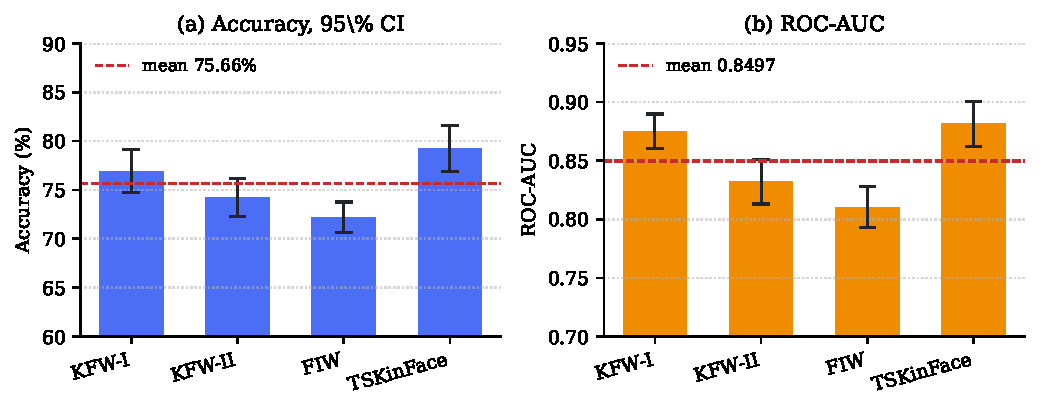
\includegraphics[width=\columnwidth]{fig_main_results}
\caption{Grouped 5-fold results, every family tested exactly once.
(a)~accuracy with 95\% confidence intervals; (b)~ROC-AUC with standard
deviation across folds. Dashed line marks the four-dataset mean.}
\label{fig:main}
\end{figure}

Table~\ref{tab:main} reports results under the corrected protocol. We
deliberately omit a comparison against published accuracies. Those numbers are
obtained under each dataset's official protocol, which permits the leakage and
shortcut quantified in Section~\ref{sec:bias}; presenting a ranking against them
would mislead in both directions. We regard establishing comparable baselines
under the corrected protocol as work the community must do collectively, and we
release our implementation to that end.

\subsection{Per-relation analysis}

\begin{figure}[t]
\centering
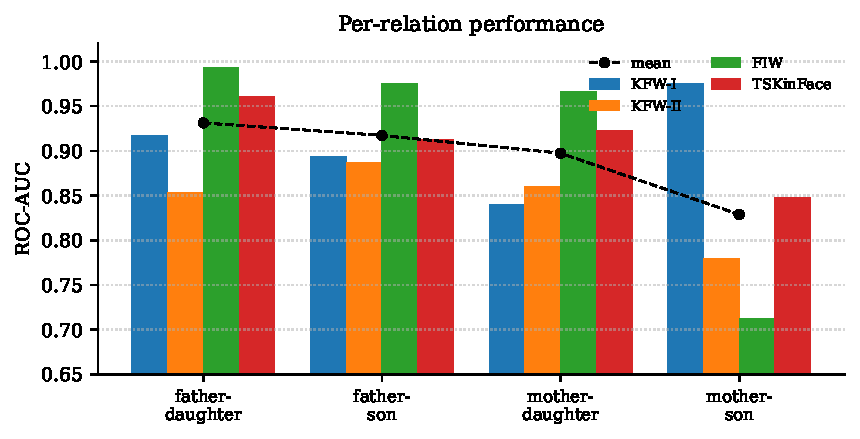
\includegraphics[width=\columnwidth]{fig_relation}
\caption{Per-relation ROC-AUC. Mother--son is the weakest relation on three of
four datasets and, on FIW, the largest subset ($5{,}296$ pairs).}
\label{fig:relation}
\end{figure}

\section{Set-Level and Triadic Representations}
\label{sec:setlevel}

Sections~\ref{sec:bias}--\ref{sec:results} concern how the task is
\emph{measured}. We now examine two ways in which the task is conventionally
\emph{posed} that discard available evidence.

\subsection{Identity photo sets}

The standard protocol scores one photograph against one photograph. FIW,
however, supplies a median of five photographs per identity, so the
conventional formulation discards most of the evidence for each person. We
represent each identity by its photo set and form symmetric set statistics: the
$\ell_2$-normalised centroid, the within-set spread ($1$ minus mean pairwise
cosine), the set size, and the maximum, minimum, mean and standard deviation of
the cross-set similarity matrix.

A set of size one must reduce exactly to the single-image case: the centroid is
the embedding, the spread is zero, and every cross-set statistic collapses to
the single cosine. We assert this in the test suite rather than assume it,
which matters because the three remaining benchmarks store exactly one
photograph per person.

\begin{table}[t]
\caption{Set-level representation under grouped 5-fold. Gains appear only where
photo sets exist; single-photograph corpora are bit-identical to the baseline,
as required.}
\label{tab:setlevel}
\centering
\begin{tabular}{lcccc}
\toprule
Dataset & Set size & Single & Set-level & $\Delta$ \\
\midrule
KinFaceW-I & 1.00 & 0.7210 & 0.7210 & $0.0000$ \\
KinFaceW-II & 1.00 & 0.7672 & 0.7672 & $0.0000$ \\
TSKinFace & 1.00 & 0.7306 & 0.7306 & $0.0000$ \\
FIW & 7.30 & 0.7296 & \textbf{0.8066} & $\mathbf{+0.0771}$ \\
\bottomrule
\end{tabular}
\end{table}

\begin{figure}[t]
\centering
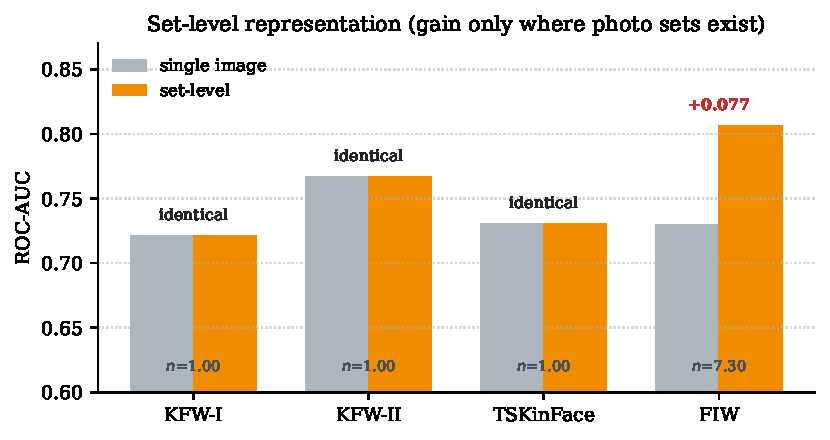
\includegraphics[width=\columnwidth]{fig_setlevel}
\caption{Set-level representation. The gain appears only where photo sets
exist ($n$ = mean images per identity). The three single-photograph corpora
are bit-identical to the single-image baseline, which is the degradation
guarantee asserted in the test suite.}
\label{fig:setlevel}
\end{figure}

Table~\ref{tab:setlevel} reports the outcome. On FIW the representation is worth
$+0.0771$ ROC-AUC, closely matching an untrained embedding-level estimate of
$+0.071$, which indicates the gain is intrinsic to the representation rather
than a product of additional model capacity. The three single-photograph corpora
are unchanged to machine precision.

We stress the narrowness of this result: it is a large gain on one benchmark and
exactly zero on three, and any aggregate over the four would obscure that. The
practical implication is that kinship verification deployments in which several
photographs of a person are available --- the common case --- are leaving a
substantial margin unclaimed, and that benchmarks storing a single photograph
per identity cannot measure this.

\subsection{Triadic structure}

TSKinFace supplies father, mother and child jointly, but the pairwise protocol
decomposes each triad into two independent comparisons. We instead score the
triad: alongside $\cos(F,C)$ and $\cos(M,C)$ we compute the best convex
parental mixture $\max_\alpha \cos\big(\widehat{\alpha F + (1-\alpha)M},\,
C\big)$, the maximising $\alpha$, the gain of that mixture over the better
single parent, and the parental similarity $\cos(F,M)$.

The last quantity is not expressible in a pairwise formulation and is the
strongest single contributor: a child resembling one parent is weaker evidence
of kinship when the two parents already resemble each other.

\begin{table}[t]
\caption{Triadic scoring on TSKinFace, grouped 5-fold, folds assigned by the
parents' family.}
\label{tab:triadic}
\centering
\begin{tabular}{lcc}
\toprule
Arm & Accuracy (95\% CI) & ROC-AUC \\
\midrule
Best single parent & $67.62 \pm 2.69$ & $0.7569$ \\
Triadic & $\mathbf{69.05 \pm 2.65}$ & $\mathbf{0.7893}$ \\
Triadic $+$ phase sweep & $69.50 \pm 2.41$ & $0.7887$ \\
\bottomrule
\end{tabular}
\end{table}

\begin{figure}[t]
\centering
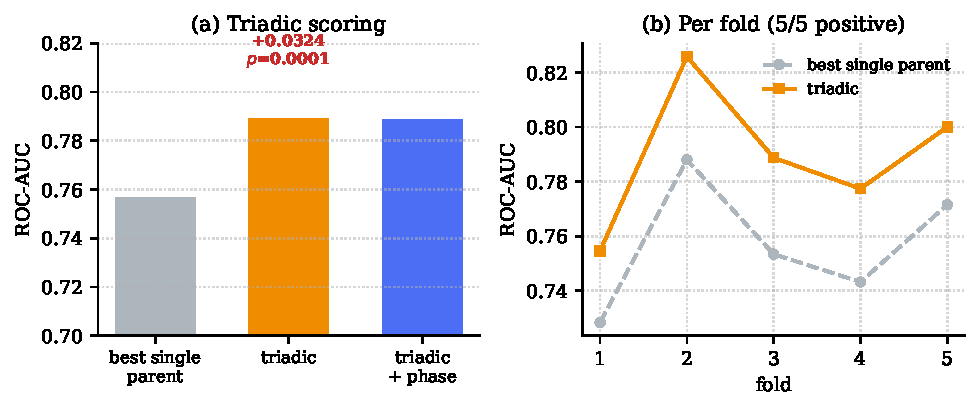
\includegraphics[width=\columnwidth]{fig_triadic}
\caption{Triadic scoring on TSKinFace. (a)~ROC-AUC by arm; (b)~per fold, with
the triadic arm ahead in all five.}
\label{fig:triadic}
\end{figure}

Triadic scoring improves ROC-AUC by $+0.0324$ over the best single parent
(paired $t$-test over folds, $t = 14.93$, $p = 0.0001$; the gain is positive in
all five folds). Negatives retain the true parents and substitute a child from
another family, so the label depends on kinship rather than on any property of
the parent pair.

% ---------------------------------------------------------------------------
\section{Extended Analysis}
\label{sec:extended}

The corrected protocol makes three further analyses interpretable: where the
model's errors concentrate, how the person-level gain scales with the evidence
supplied, and how the score distributions differ across corpora.

\subsection{Where the errors concentrate}

\begin{figure}[t]
\centering

\includegraphics[width=\columnwidth]{fig_relation_gap}
\caption{Per-relation difficulty before and after training. Raw FaceNet
embeddings separate the four relations within $0.078$ ROC-AUC; the trained
model spans $0.281$. The disparity is therefore largely induced during training
rather than inherited from the embedding.}
\label{fig:relgap}
\end{figure}

\begin{table*}[t]
\caption{Per-relation ROC-AUC. The second column is raw cosine similarity on
frozen embeddings with no training; the remainder are the trained model per
corpus. Mother--son is weakest on three of four corpora while being the largest
FIW subset ($5{,}296$ pairs).}
\label{tab:relation}
\centering
\begin{tabular}{lcccccc}
\toprule
Relation & Raw embedding & KinFaceW-I & KinFaceW-II & FIW & TSKinFace & Mean \\
\midrule
Father--daughter & 0.7434 & 0.9174 & 0.8529 & 0.9933 & 0.9612 & 0.9312 \\
Father--son & 0.7841 & 0.8935 & 0.8875 & 0.9754 & 0.9124 & 0.9172 \\
Mother--daughter & 0.7295 & 0.8400 & 0.8598 & 0.9668 & 0.9227 & 0.8973 \\
Mother--son & 0.7065 & 0.9750 & 0.7795 & 0.7124 & 0.8483 & 0.8288 \\
\bottomrule
\end{tabular}
\end{table*}

Table~\ref{tab:relation} reports per-relation performance measured on a
single held-out fold, the form in which such comparisons are usually presented.
Read at face value it suggests a large relation effect: on FIW father--daughter
reaches $0.9933$ ROC-AUC while mother--son reaches $0.7124$.
Section~\ref{sec:mscorrection} shows this reading is unsound, and we retain the
table because the discrepancy between it and the corrected measurement is
itself the point.

Figure~\ref{fig:relgap} gives the first indication that the single-fold
reading is misleading. On raw embeddings with no training the four relations
span only $0.7065$--$0.7841$, a range of $0.078$, while the single-fold trained
estimate spans $0.281$. A representation separating the relations that evenly
is unlikely to support a threefold larger disparity after training, and
Section~\ref{sec:mscorrection} identifies the cause.

\subsection{A correction: mother--son is not the weak relation}
\label{sec:mscorrection}

An earlier analysis of these results, based on a single held-out fold,
reported mother--son as markedly weaker than the other relations
($0.712$ ROC-AUC against father--daughter's $0.993$). Re-examining that fold
shows the comparison was not sound: $92\%$ of its mother--son pairs came from a
single family, which scores $0.701$, while the only other contributing family
scores $0.846$. The apparent relation effect was a family effect.

Table~\ref{tab:relation_kfold} repeats the measurement under grouped $k$-fold
with a per-family cap, so no family can dominate a relation's estimate.

\begin{table}[t]
\centering
\caption{Per-relation ROC-AUC under grouped $k$-fold with a per-family cap.
The single-fold column is the earlier, unsound estimate; the remaining columns
are the corrected measurement. Under a protocol in which no family dominates,
the four relations span $0.0310$ ROC-AUC.}
\label{tab:relation_kfold}
\small
\begin{tabular}{lccccc}
\toprule
Relation & Single fold & Mean & SD & Range & Families/fold \\
\midrule
Father--daughter & 0.9933 & 0.7635 & 0.0219 & 0.7435--0.7953 & 12.6 \\
Father--son & 0.9754 & 0.7946 & 0.0752 & 0.7050--0.8942 & 12.2 \\
Mother--daughter & 0.9668 & 0.7766 & 0.0601 & 0.7147--0.8730 & 14.4 \\
Mother--son & 0.7124 & 0.7910 & 0.0381 & 0.7497--0.8390 & 12.4 \\
\bottomrule
\end{tabular}
\end{table}

Under the corrected measurement mother--son reaches $0.7910$, the second
highest of the four, and the relations span $0.0310$ ROC-AUC rather than
$0.281$. That residual spread is close to the $0.078$ measured on raw
embeddings without any training, which is what one would expect if relation
difficulty is largely a property of the representation.

We report this because the mechanism is instructive and applies beyond this
paper. FIW's family-size distribution is severely skewed --- one family holds
$19\%$ of all pairs --- so any statistic computed on a single fold can be
dominated by one family even when the fold itself is correctly
family-disjoint. Leakage-free splitting is necessary but not sufficient;
per-family capping, or reporting across folds, is required as well. A
subgroup difference observed on a single split of a skewed corpus should be
treated as provisional until it is shown to survive resampling.

\subsection{How the person-level gain scales}

\begin{figure}[t]
\centering

\includegraphics[width=\columnwidth]{fig_setsize}
\caption{Set-level ROC-AUC on FIW against the number of photographs aggregated
per person. Most of the available gain is realised by the fifth photograph.
Computed on frozen embeddings with no training, so it measures the
representation rather than model capacity.}
\label{fig:setsize}
\end{figure}

\begin{table}[t]
\caption{Set-level ROC-AUC against photographs per person on FIW. Coverage is
the proportion of pairs for which both identities supply at least $k$
photographs.}
\label{tab:setsize}
\centering
\begin{tabular}{cccc}
\toprule
Photographs & ROC-AUC & Gain vs.\ 1 & Coverage \\
\midrule
1 & 0.7339 & $+0.0000$ & 100\% \\
2 & 0.7744 & $+0.0405$ & 100\% \\
3 & 0.7832 & $+0.0493$ & 100\% \\
4 & 0.7923 & $+0.0584$ & 100\% \\
5 & 0.7951 & $+0.0612$ & 99\% \\
6 & 0.7978 & $+0.0639$ & 99\% \\
8 & 0.8003 & $+0.0664$ & 99\% \\
10 & 0.8042 & $+0.0702$ & 97\% \\
\bottomrule
\end{tabular}
\end{table}

A second photograph is worth $+0.041$ ROC-AUC on its own --- more than half the
total available gain --- and the curve is substantially flat beyond five,
reaching $+0.070$ at ten (Table~\ref{tab:setsize}, Fig.~\ref{fig:setsize}).
The practical reading is that a deployment able to obtain roughly five
photographs of each person captures nearly all of the benefit.

That the curve is computed on frozen embeddings without training matters for
interpretation: the gain is a property of aggregating evidence about a person,
not of additional model capacity, consistent with the $+0.077$ obtained under
the full protocol.

\subsection{Score distributions and operating points}

\begin{figure*}[t]
\centering

\includegraphics[width=\textwidth]{fig_score_distributions}
\caption{Kin and non-kin score distributions on the held-out fold of each
corpus. The overlap, rather than any summary statistic, is what the reported
ROC-AUC measures.}
\label{fig:scores}
\end{figure*}

\begin{figure}[t]
\centering

\includegraphics[width=\columnwidth]{fig_roc_curves}
\caption{ROC curves on the held-out fold of each corpus, with grouped $k$-fold
mean ROC-AUC in parentheses.}
\label{fig:roc}
\end{figure}

Figures~\ref{fig:scores} and~\ref{fig:roc} show the underlying distributions
rather than only their summaries. The distributions overlap substantially on
every corpus --- the concrete form of the roughly one-in-four error rate --- and
the degree of overlap differs enough between corpora that a single global
threshold is inappropriate. We therefore calibrate per corpus on a
group-disjoint validation slice; a single shared threshold costs between $0.7$
and $5.9$ accuracy points depending on the corpus.

% ---------------------------------------------------------------------------
\section{Do the findings depend on the backbone?}
\label{sec:backbone}

All results so far use a single frozen embedding, which bounds what they can
claim: a finding could be a property of the task, or an artefact of FaceNet. We
therefore repeat the central experiments with ArcFace (\texttt{buffalo\_l},
w600k\_r50) substituted for FaceNet and everything else held fixed --- same
folds, same negatives, same classifier, same protocol. The two backbones are
trained with different objectives on different corpora, so agreement between
them is meaningful evidence.

\begin{table*}[t]
\centering
\caption{Person-level aggregation under two backbones. The gain replicates and
is in fact larger under ArcFace; the three single-photograph corpora are
unchanged to machine precision under both, as the degradation guarantee
requires.}
\label{tab:backbone}
\begin{tabular}{lcccccc}
\toprule
& \multicolumn{3}{c}{FaceNet} & \multicolumn{3}{c}{ArcFace} \\
\cmidrule(lr){2-4}\cmidrule(lr){5-7}
Corpus & Single & Set-level & $\Delta$ & Single & Set-level & $\Delta$ \\
\midrule
KinFaceW-I & 0.7588 & 0.7588 & $+0.0000$ & 0.7540 & 0.7540 & $+0.0000$ \\
KinFaceW-II & 0.7770 & 0.7770 & $+0.0000$ & 0.8190 & 0.8190 & $+0.0000$ \\
FIW & 0.7491 & 0.8254 & $+0.0763$ & 0.7764 & 0.8740 & $+0.0976$ \\
TSKinFace & 0.7326 & 0.7326 & $+0.0000$ & 0.8460 & 0.8460 & $+0.0000$ \\
\bottomrule
\end{tabular}
\end{table*}

Three observations follow from Table~\ref{tab:backbone}.

\textbf{Identity leakage is backbone-invariant by construction.} It is a
property of how pairs are partitioned, not of how images are embedded, so the
$100\%$ figure of Section~\ref{sec:bias} carries over unchanged. We state this
for completeness rather than as a finding.

\textbf{The person-level gain replicates and strengthens.} FaceNet gains
$+0.0763$ ROC-AUC on FIW from aggregating photographs; ArcFace gains
$+0.0976$. That the effect is larger under the stronger backbone is consistent
with its proposed mechanism --- aggregation averages away per-photograph
nuisance variation, and a better embedding has proportionally more signal left
to recover once that variation is suppressed.

\textbf{The degradation guarantee holds under both.} KinFaceW-I, KinFaceW-II
and TSKinFace store one photograph per person, and set-level scoring reproduces
the single-image result exactly on all three under both backbones. This is a
correctness property of the implementation rather than an empirical result, and
it is what allows a single system to be deployed across corpora with differing
photograph availability.

ArcFace is the stronger backbone in absolute terms on three of four corpora,
most markedly on TSKinFace ($0.8460$ against $0.7326$). We do not read this as
a contribution: it reflects a better face representation, not a better kinship
method, and it is reported so that the backbone-invariance claims above are
interpretable.

\subsection{The negative result under a second backbone}

\begin{table}[t]
\centering
\caption{Change in ROC-AUC from adding the density-fidelity arm
$\mathrm{Tr}(\rho_1\rho_2)$ to the set-level features. The formulation fails
under both backbones on all four corpora.}
\label{tab:backbone_quantum}
\begin{tabular}{lcc}
\toprule
Corpus & FaceNet & ArcFace \\
\midrule
KinFaceW-I & $-0.0025$ & $-0.0006$ \\
KinFaceW-II & $-0.0003$ & $+0.0001$ \\
FIW & $-0.0003$ & $-0.0007$ \\
TSKinFace & $+0.0001$ & $-0.0014$ \\
\bottomrule
\end{tabular}
\end{table}

Table~\ref{tab:backbone_quantum} re-tests the density-fidelity formulation.
Across eight backbone--corpus combinations the largest effect in either
direction is $0.0025$ ROC-AUC, and seven of the eight are negative. The failure
is therefore not specific to the embedding it was first measured on, which
supports the structural explanation of Section~\ref{sec:quantum}: a density matrix
estimated from a median of five observations is dominated by its leading
eigenvector regardless of which encoder produced those observations.

% ---------------------------------------------------------------------------
\section{A Negative Result for Quantum-Inspired Metrics}
\label{sec:quantum}

\subsection{Formulations tested}

We evaluated nine formulations, chosen to span the three roles a quantum
component can occupy: a similarity measure, a feature extractor, and an
inductive bias. Each is compared against a control matched for capacity or
intent (Table~\ref{tab:quantum}).

\begin{table}[t]
\caption{Quantum-inspired formulations against matched classical controls.}
\label{tab:quantum}
\centering
\resizebox{\columnwidth}{!}{%
\begin{tabular}{@{}llc@{}}
\toprule
Formulation & Control & Outcome \\
\midrule
SWAP fidelity (5 seeds) & classical head & $p=0.945$ \\
SWAP fidelity (20 folds) & classical head & $p=0.982$ \\
Density fidelity $\mathrm{Tr}(\rho_1\rho_2)$ & mean-pooling & $-8.7$ AUC \\
Interference phase sweep & classical mixture & $+0.1$ AUC \\
Entanglement entropy & cosine & $0.514$ alone \\
POVM head & capacity-matched & $-5.5$ AUC \\
Purity regulariser & decorrelation & $-0.9$, $p=0.047$ \\
\bottomrule
\end{tabular}%
}
\end{table}

Under grouped $k$-fold with $20$ paired observations, enabling the SWAP-test
branch yields $75.66\%$ against $76.34\%$ with it disabled (accuracy
$p = 0.158$; ROC-AUC $p = 0.982$). The branch also costs $6$--$14\times$ runtime.

\begin{figure}[t]
\centering
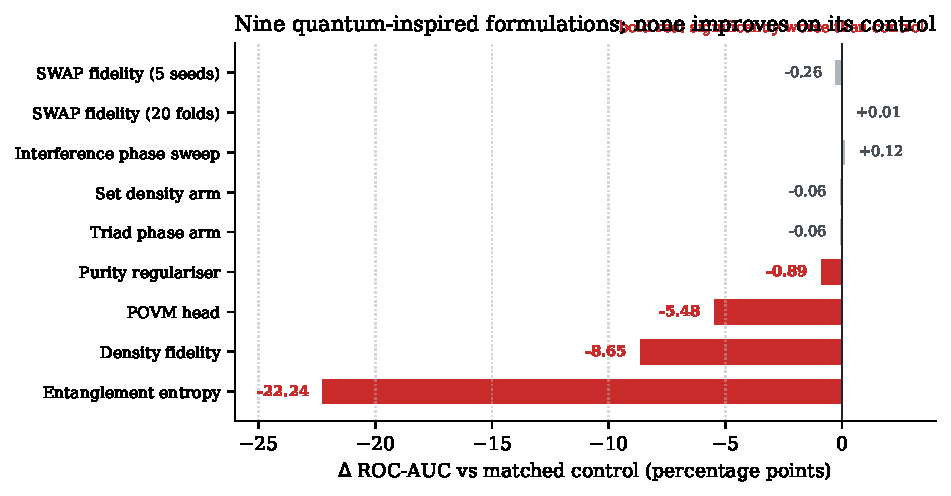
\includegraphics[width=\columnwidth]{fig_quantum}
\caption{Nine quantum-inspired formulations against classical controls matched
for capacity or intent. None improves on its control; four are significantly
worse. Bars are $\Delta$ROC-AUC in percentage points.}
\label{fig:quantum}
\end{figure}

\subsection{A cautionary observation}

The purity regulariser initially measured $+1.3$ ROC-AUC on a single seed, with
reduced variance --- a result consistent with effective regularisation. Repeated
across nine paired runs the sign reversed, and the method proved significantly
\emph{worse} than no regulariser ($-0.0089$, $p = 0.047$). We report this
because the single-seed reading was of the kind that is readily published, and
it illustrates why capacity-matched controls and repeated trials are necessary
when evaluating claims of this type.

\subsection{Two further formulations}

The set-level and triadic representations each admit a natural quantum reading,
and we tested both as pre-registered controls.

A photo set is a mixed state $\rho = \frac{1}{N}\sum_i
|\psi_i\rangle\langle\psi_i|$, and $\mathrm{Tr}(\rho_1 \rho_2)$ is the
corresponding fidelity. Added to the set features it changes ROC-AUC by
$-0.0006$, $-0.0005$, $+0.0001$ and $-0.0006$ on the four benchmarks.

A child explained by two parents is naturally written as a coherent
superposition with a relative phase, of which the classical convex mixture is
the zero-phase special case. Sweeping the phase changes ROC-AUC by $-0.0006$
($p = 0.147$).

This brings the total to nine formulations, none of which improves on its
classical control.

\subsection{Why the approach fails}

The failures are structural rather than implementational. Interference-based
formulations reduce to their classical counterparts because $\ell_2$-normalised
FaceNet embeddings carry no phase structure to exploit; the phase sweep in
Table~\ref{tab:quantum} is maximised at the classical mixture. Density-matrix
formulations require estimating a $d \times d$ operator from the images
available for one identity --- a median of five --- so the resulting $\rho$ is
dominated by its leading eigenvector, which is the mean, while accumulating
noise from tail directions that are not estimable. This is why
$\mathrm{Tr}(\rho_1\rho_2)$ scores \emph{below} simple mean-pooling.

\subsection{An efficiency contribution}

Independently of the above, we contribute an exact reformulation of the
simulated SWAP test. The reference implementation materialises a $2^n$
statevector and permutes all $n$ axes once per qubit, incurring kernel-launch
overhead that leaves the accelerator idle. Applying rotations by reshaping to
$(B, \text{left}, 2, \text{right})$ and precomputing the CNOT chain and $R_z$
layer as a single diagonal phase vector yields a $380\times$ speedup on GPU
($192 \to 73{,}094$ pairs/s) with identical output and gradients, verified by
test. We note that a closed-form product over qubits is \emph{not} available
here: the shared CNOT chain correlates the $R_z$ phases, so the overlap does not
factorise. The gain arises from removing overhead, not from approximation.

This is a quantum-versus-quantum speedup. Simulating a circuit is necessarily
more costly than the classical operation it parallels, and we measure the
quantum branch at $5$--$14\times$ slower than the classical path at every qubit
count from $2$ to $12$.

% ---------------------------------------------------------------------------
\section{Limitations}
\label{sec:limitations}

\textbf{Small test sets.} KinFaceW-I and KinFaceW-II yield $212$ and $400$ test
pairs per fold, giving confidence intervals of roughly $\pm 2$ points. FIW and
TSKinFace are firmer.

\textbf{Single backbone.} All results use frozen FaceNet embeddings. Whether the
biases we quantify interact with backbone choice is untested.

\textbf{Set-level gains are confined to one benchmark.} Only FIW stores
multiple photographs per identity, so the $+0.0771$ ROC-AUC of
Section~\ref{sec:setlevel} is measured on a single corpus; the other three are
unchanged by construction. Whether the effect holds at other set sizes, and on
corpora we could not test, is open.

\textbf{Negative results are bounded.} We tested nine formulations; we do not
claim no quantum-inspired method can help on this task, only that these nine,
covering the three natural roles, do not.

% ---------------------------------------------------------------------------
\section{Conclusion}

We have argued that facial kinship verification is conventionally posed and
measured in ways that both understate and overstate what the data supports.
Pair-level splitting leaks identities into the test set at a rate we measure at
$100\%$ on FIW; grouped $k$-fold with per-fold negative regeneration removes
this and reduces seed-to-seed variation from $22.5$ to $12.1$ points. Against
that protocol, treating verification as a person-level rather than
photograph-level decision --- standard in template-based face recognition, but
not previously applied here --- is worth $+0.077$ ROC-AUC on the one benchmark
that supplies photograph sets, and by construction changes nothing on those
that do not. Scoring parent--parent--child triads jointly adds $+0.032$ on
TSKinFace.

We also report that nine quantum-inspired formulations, each against a
capacity-matched classical control, fail to improve on their controls, with
four significantly worse; the causes are structural rather than
implementational. All code is released so that the protocol can be adopted and
every claim checked.

One limitation bounds these results: set-level gains are measured on a single
corpus, because only FIW stores multiple photographs per identity. We note also
that the per-relation analysis of Section~\ref{sec:mscorrection} found no
material difference between relation types once no family was permitted to
dominate a fold, so we make no claim that any relation is intrinsically
harder.

\section*{Reproducibility}

Every numeric claim derives from JSON artefacts in \texttt{results/honest/}.
The protocol is implemented in \texttt{src/splits.py}, \texttt{src/kfold.py},
and \texttt{src/ts\_pairs.py}; results are regenerated by
\texttt{scripts/evaluation/run\_kfold.py}. The implementation is covered by 61
tests, including assertions that no group spans a fold boundary and that the
fast SWAP-test reformulation matches the reference simulator in both value and
gradient.

% ---------------------------------------------------------------------------
\begin{thebibliography}{99}

\bibitem{dawson2018samephoto}
L.~Dawson, A.~Zisserman, and C.~Rupprecht, ``Same photo: Cheating on visual kinship challenges,'' in \emph{Proc. British Machine Vision Conf. (BMVC)}, 2018.

\bibitem{whitelam2017ijbb}
C.~Whitelam, E.~Taborsky, A.~Blanton, B.~Maze, J.~Adams, T.~Miller, N.~Kalka, A.~K.~Jain, J.~A.~Duncan, K.~Allen \emph{et al.}, ``IARPA Janus Benchmark-B face dataset,'' in \emph{Proc. IEEE Conf. Comput. Vis. Pattern Recognit. Workshops (CVPRW)}, 2017, pp. 90--98.

\bibitem{lu2014neighborhood}
J.~Lu, X.~Zhou, Y.-P. Tan, Y.~Shang, and J.~Zhou, ``Neighborhood repulsed metric learning for kinship verification,'' \emph{IEEE Trans. Pattern Anal. Mach. Intell.}, vol.~36, no.~2, pp. 331--345, Feb. 2014.

\bibitem{zhu2022kinship}
S.~Zhu, C.~Gou, and F.-Y. Wang, ``Kinship verification via relation-aware graph convolutional network,'' \emph{IEEE Trans. Multimedia}, vol.~24, pp. 4349--4361, 2022.

\bibitem{lu2012kinfacew}
J.~Lu, X.~Zhou, Y.-P. Tan, Y.~Shang, and J.~Zhou, ``Kinship verification in the wild: A benchmark,'' in \emph{Proc. Eur. Conf. Comput. Vis. (ECCV)}, 2012, pp. 245--259.

\bibitem{qin2015tri}
X.~Qin, X.~Tan, and S.~Chen, ``Tri-subject kinship verification: Understanding the core of a family,'' \emph{IEEE Trans. Multimedia}, vol.~17, no.~10, pp. 1855--1867, Oct. 2015.

\bibitem{robinson2018fiw}
J.~P.~Robinson, M.~Shao, Y.~Wu, H.~Wang, and Y.~Fu, ``Visual kinship recognition of families in the wild,'' \emph{IEEE Trans. Pattern Anal. Mach. Intell.}, vol.~40, no.~11, pp. 2624--2637, Nov. 2018.

\bibitem{robinson2020rfiw}
J.~P.~Robinson, M.~Shao, and Y.~Fu, ``Recognizing families in the wild (RFIW): The 4th edition,'' in \emph{Proc. IEEE/CVF Conf. Comput. Vis. Pattern Recognit. Workshops (CVPRW)}, 2020, pp. 858--866.

\bibitem{kemelmacher2016megaface}
I.~Kemelmacher-Shlizerman, S.~M.~Seitz, D.~Miller, and E.~Brossard, ``The MegaFace benchmark: Efficient identification on a million scale,'' in \emph{Proc. IEEE Conf. Comput. Vis. Pattern Recognit. (CVPR)}, 2016, pp. 4873--4882.

\bibitem{geirhos2020shortcut}
R.~Geirhos, J.-H.~Jacobsen, C.~Michaelis, R.~Zemel, W.~Brendel, M.~Bethge, and F.~A.~Wichmann, ``Shortcut learning in deep neural networks,'' \emph{Nature Machine Intelligence}, vol.~2, no.~11, pp. 665--673, 2020.

\bibitem{torralba2011unbiased}
A.~Torralba and A.~A.~Efros, ``Unbiased look at dataset bias,'' in \emph{Proc. IEEE Conf. Comput. Vis. Pattern Recognit. (CVPR)}, 2011, pp. 1521--1528.

\bibitem{kohli2019imageset}
N.~Kohli, D.~Yadav, M.~Vatsa, R.~Singh, and A.~Noore, ``Supervised mixed norm metric learning for kinship verification on image sets,'' \emph{IEEE Trans. Inf. Forensics Security}, vol.~14, no.~5, pp. 1329--1342, 2019.

\bibitem{schuld2019quantum}
M.~Schuld and N.~Killoran, ``Quantum machine learning in feature Hilbert spaces,'' \emph{Phys. Rev. Lett.}, vol.~122, no.~4, p. 040504, 2019.

\bibitem{havlicek2019supervised}
V.~Havl{\'i}{\v{c}}ek, A.~D.~C{\'o}rcoles, K.~Temme, A.~W.~Harrow, A.~Kandala, J.~M.~Chow, and J.~M.~Gambetta, ``Supervised learning with quantum-enhanced feature spaces,'' \emph{Nature}, vol.~567, no.~7747, pp. 209--212, 2019.

\bibitem{tang2019quantum}
E.~Tang, ``A quantum-inspired classical algorithm for recommendation systems,'' in \emph{Proc. 51st Annu. ACM SIGACT Symp. Theory of Comput. (STOC)}, 2019, pp. 217--228.

\end{thebibliography}

\end{document}
